\chapter{Results}
This chapter gives the results of various benchmarks performed on StreamingATLOD.
Two types of benchmarks are performed.
The first type are 5 flight experiments,
whose main goal is to benchmark how much time StreamingATLOD 
needs to stream in new data when the disk cache is empty
and how well StreamingATLOD performs in terms of rendering performance.
A single flying experiment consists of a simple 
flight starting from outer space towards a destination on the Earth and aims to show the following:
\begin{itemize}
  \item A screenshot of the destination place at the highest available resolution.
  \item The number of requests StreamingATLOD performs when flying to a place for the first time
  and the amount of time it requires until loading all required data, including the time 
  between arriving at the destination and receiving the last API response.
  \item The average framerate of such a flight.
  \item The number of traversed terrain nodes, draw calls and rendered triangles when vieweing the destination place (at the state of the screenshot).
  \item The total memory consumption done by StreamingATLOD when viewing the destination place.
\end{itemize}
As such, all flight experiments were conducted with the disk cache empty upon every start up.
The time measurements were performed manually with a stopwatch app on a mobile phone 
since the time differences are in the range of multiple seconds.
The total memory consumption (CPU + GPU) is retrieved 
from the ``Activity Monitor'' app on macOS.

The second type of benchmarking performed is the measurement 
of the disk cache size for various disk cache capacities.
Since the overlay and heightmap tiles are encoded in JPG and WebP on the disk respectively,
not all tiles use up the same amount of memory.

\section{Experimental Setup}
\subsection{Used Hardware}
The used hardware is a MacBook Air 2020 with an Intel CPU.
The specifications are displayed in table \ref{tbl:specs}.

\begin{table}[H]
  \begin{center}
    \begin{tabular}{ c|c }
      CPU & 1.1 GHz Dual-Core Intel Core i3\\
      \hline
      Memory & 8 GB 3733 MHz LPDDR4X\\
      \hline
      Graphics & Intel Iris Plus Graphics 1536 MB\\
      \hline
      OS & macOS Monterey Version 12.6\\
      \hline
      Resolution & $2560 \times 1600$
    \end{tabular}
  \end{center}
  \caption{The specifications of the used MacBook Air 2020.}\label{tbl:specs}
  \end{table}

\subsection{Application Configuration}
The application uses the following configuration settings:
\begin{itemize}
  \item Low resolution mesh size: 8
  \item Medium resolution mesh size: 32
  \item High resolution mesh size: 32
  \item Number of load worker threads: 6
  \item Heightmap data set: MapTiler RGB
  \item Overlay data set: MapTiler Satellite
  \item Memory cache size: 400 nodes
  \item Disk cache size: for the flight experiments 8000 nodes, for the disk cache measurements 400, 2000 and 8000 nodes
\end{itemize}
The application window resolution is set to $1280 \times 720$.
\pagebreak

\section{Flight Experiments}
\subsection{Experiment 1: The Swiss Alps}
\begin{figure}[H]
  \centering
  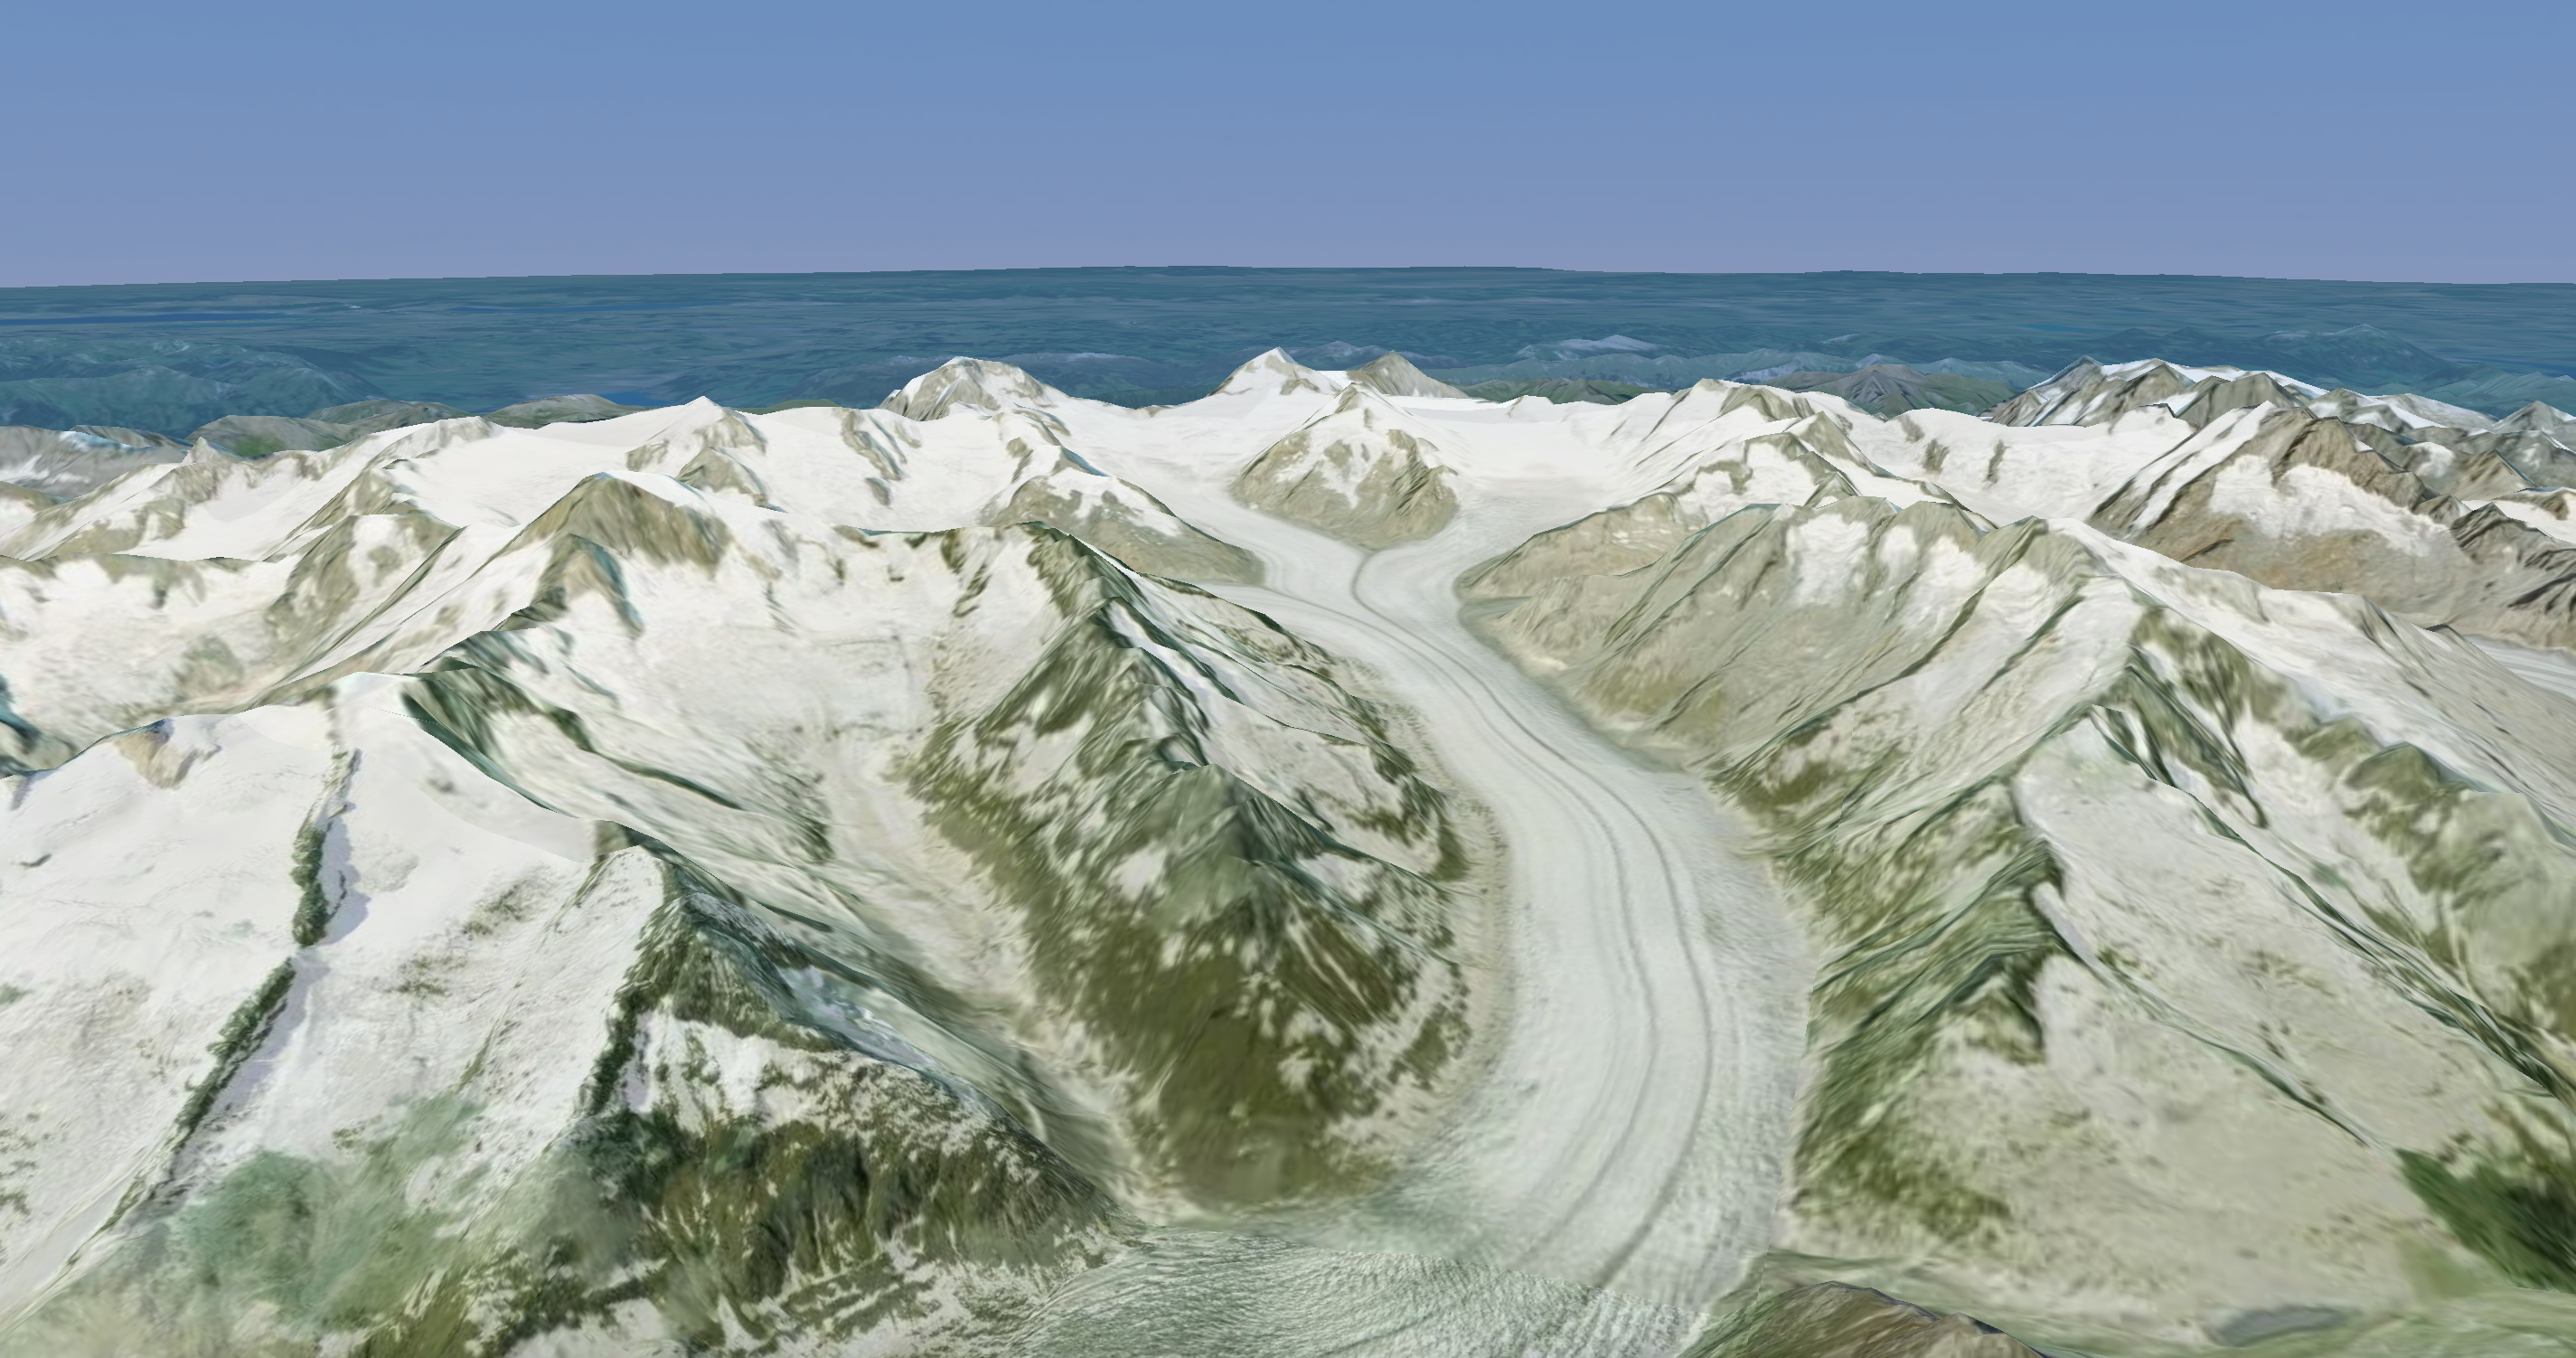
\includegraphics[width=1\textwidth]{results-screenshot-1.png}
  \caption{Screenshot of experiment 1: The Swiss Alps.}\label{fig:results-screenshot-1}
\end{figure}

\begin{table}[H]
  \begin{center}
    \begin{tabular}{ c|c }
      Time until destination reached $t_{dest}$ & 29 seconds \\
      \hline
      Time until all tiles loaded $t_{load}$ & 38 seconds\\
      \hline
      $t_{load} - t_{dest}$ & 9 seconds \\
      \hline
      Draw calls & 126 \\
      \hline
      Rendered triangles & 86002 \\
      \hline
      Visible nodes & 62 \\
      \hline
      Traversed nodes & 233 \\
      \hline
      Highest zoom level & 13 \\
      \hline
      Nodes in memory cache & 233 \\
      \hline
      Average FPS & 64.2 \\
      \hline 
      API requests & 466 \\
      \hline
      GPU memory for textures &  426.9 MB\\
      \hline
      Total memory (CPU + GPU) consumption & 901.5 MB \\
    \end{tabular}
  \end{center}
  \caption{Benchmarks for experiment 1.}\label{tbl:results-1}
  \end{table}

\subsection{Experiment 2: The Grand Canyon}
\begin{figure}[H]
  \centering
  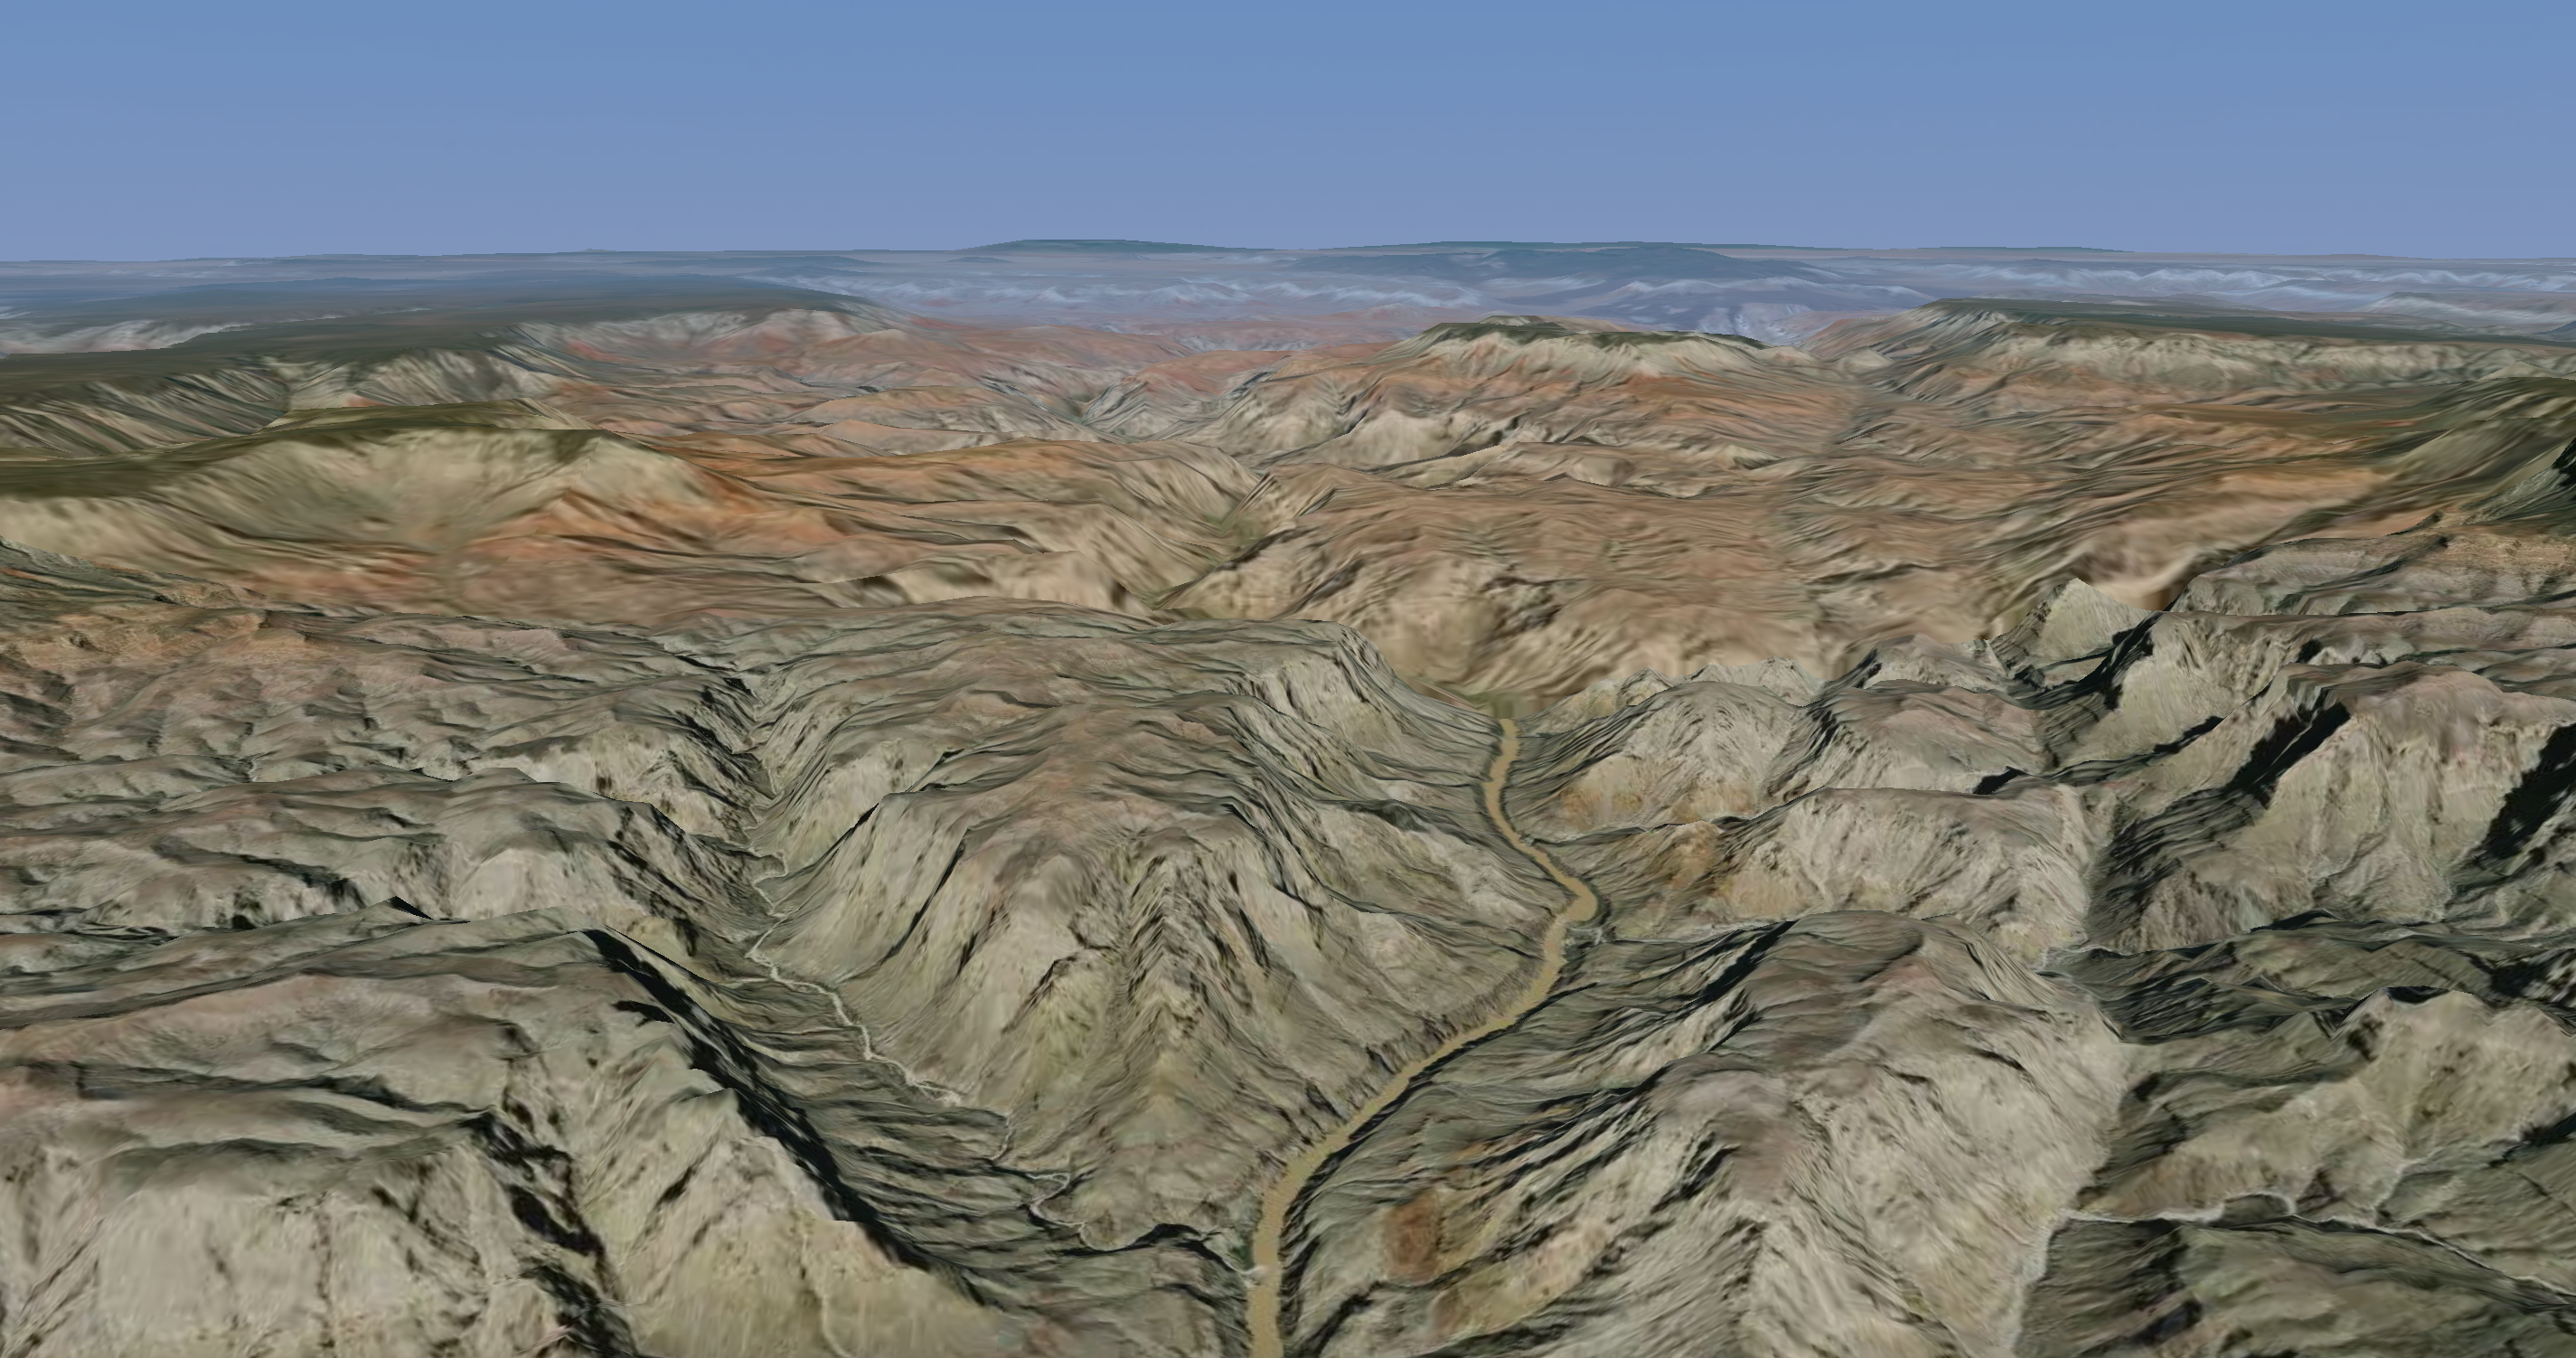
\includegraphics[width=1\textwidth]{results-screenshot-2.png}
  \caption{Screenshot of experiment 2: The Grand Canyon.}\label{fig:results-screenshot-2}
\end{figure}

\begin{table}[H]
  \begin{center}
    \begin{tabular}{ c|c }
      Time until destination reached $t_{dest}$ & 35 seconds \\
      \hline
      Time until all tiles loaded $t_{load}$ & 45 seconds \\
      \hline
      $t_{load} - t_{dest}$ & 10 seconds \\
      \hline
      Draw calls & 118 \\
      \hline
      Rendered triangles & 75422 \\
      \hline
      Visible nodes & 58 \\
      \hline
      Traversed nodes & 107 \\
      \hline
      Highest zoom level & 13 \\
      \hline
      Nodes in memory cache & 217 \\
      \hline
      Average FPS & 71.2 \\
      \hline 
      API requests & 490 \\
      \hline
      GPU memory for textures & 397.6 MB \\
      \hline
      Total memory (CPU + GPU) consumption & 824.4 MB \\
    \end{tabular}
  \end{center}
  \caption{Benchmarks for experiment 2.}\label{tbl:results-2}
  \end{table}

\subsection{Experiment 3: Northern Iceland}
\begin{figure}[H]
  \centering
  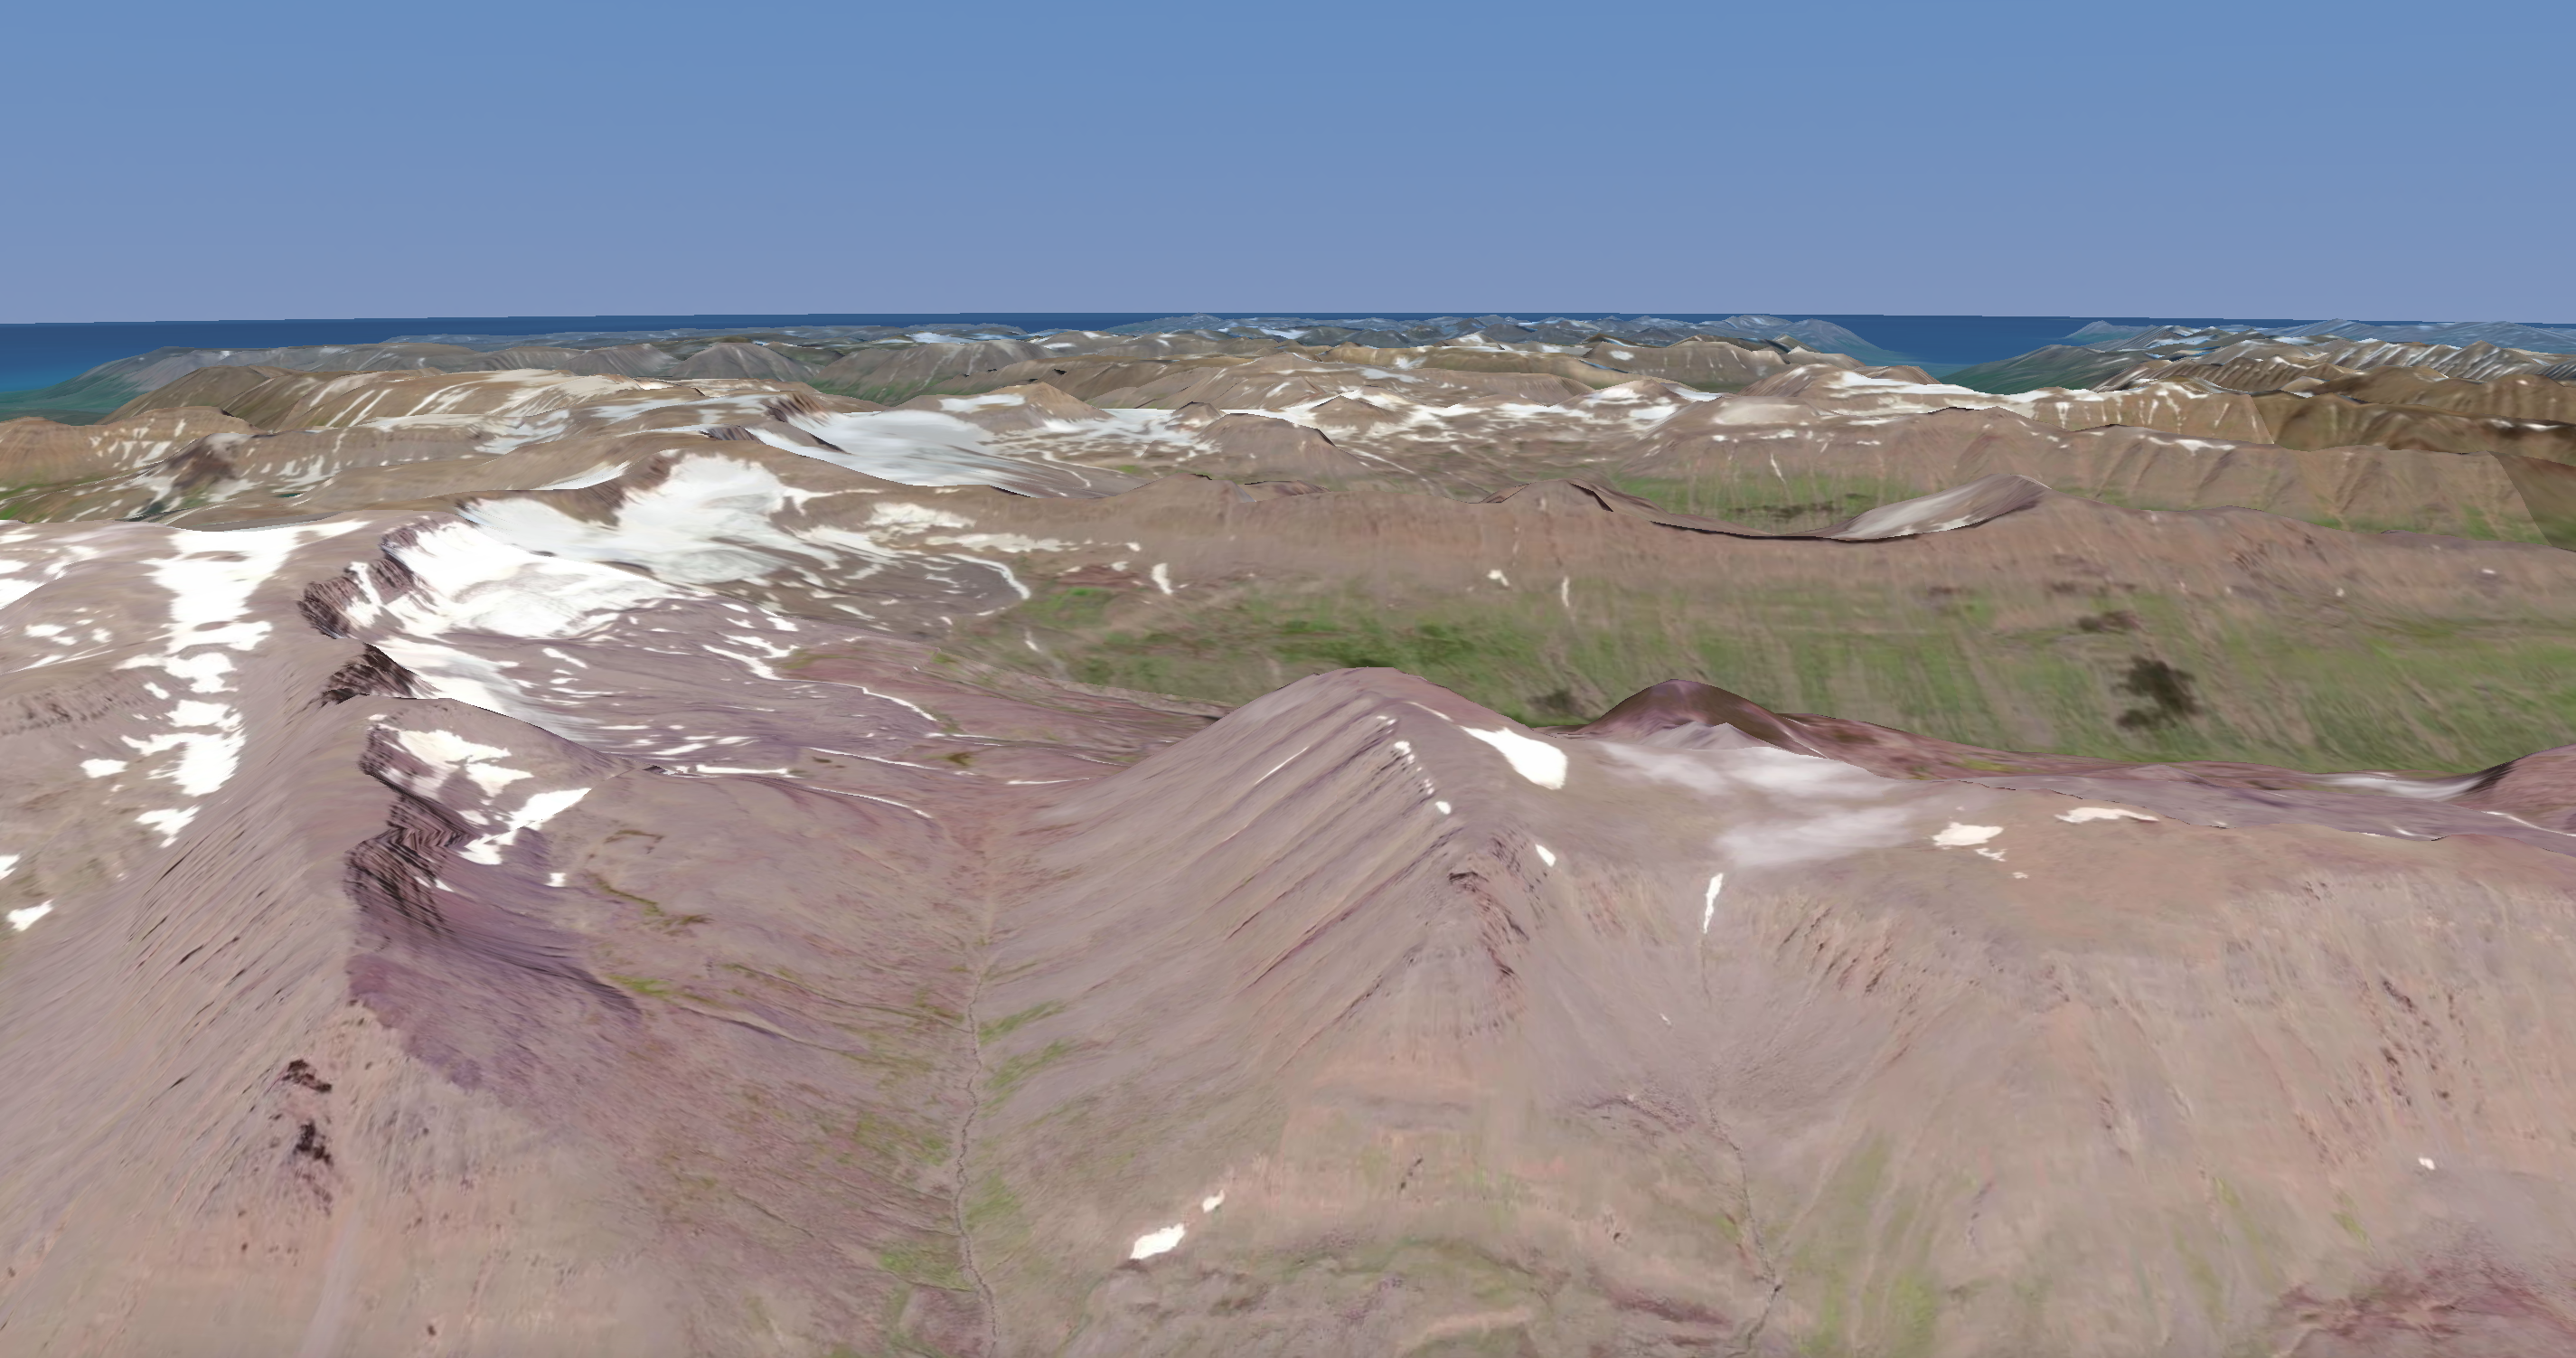
\includegraphics[width=1\textwidth]{results-screenshot-3.png}
  \caption{Screenshot of experiment 3: Northern Iceland.}\label{fig:results-screenshot-3}
\end{figure}

\begin{table}[H]
  \begin{center}
    \begin{tabular}{ c|c }
      Time until destination reached $t_{dest}$ & 35 seconds \\
      \hline
      Time until all tiles loaded $t_{load}$ & 66 seconds \\
      \hline
      $t_{load} - t_{dest}$ & 31 seconds\\
      \hline
      Draw calls & 214 \\
      \hline
      Rendered triangles & 151070 \\
      \hline
      Visible nodes & 106 \\
      \hline
      Traversed nodes & 182 \\
      \hline
      Highest zoom level & 14 \\
      \hline
      Nodes in memory cache & 309 \\
      \hline
      Average FPS & 56.4 \\
      \hline 
      API requests & 628 \\
      \hline
      GPU memory for textures & 566.2 MB \\
      \hline
      Total memory (CPU + GPU) consumption & 1.13 GB \\
    \end{tabular}
  \end{center}
  \caption{Benchmarks for experiment 3.}\label{tbl:results-3}
  \end{table}

\subsection{Experiment 4: The Andes Mountains}
\begin{figure}[H]
  \centering
  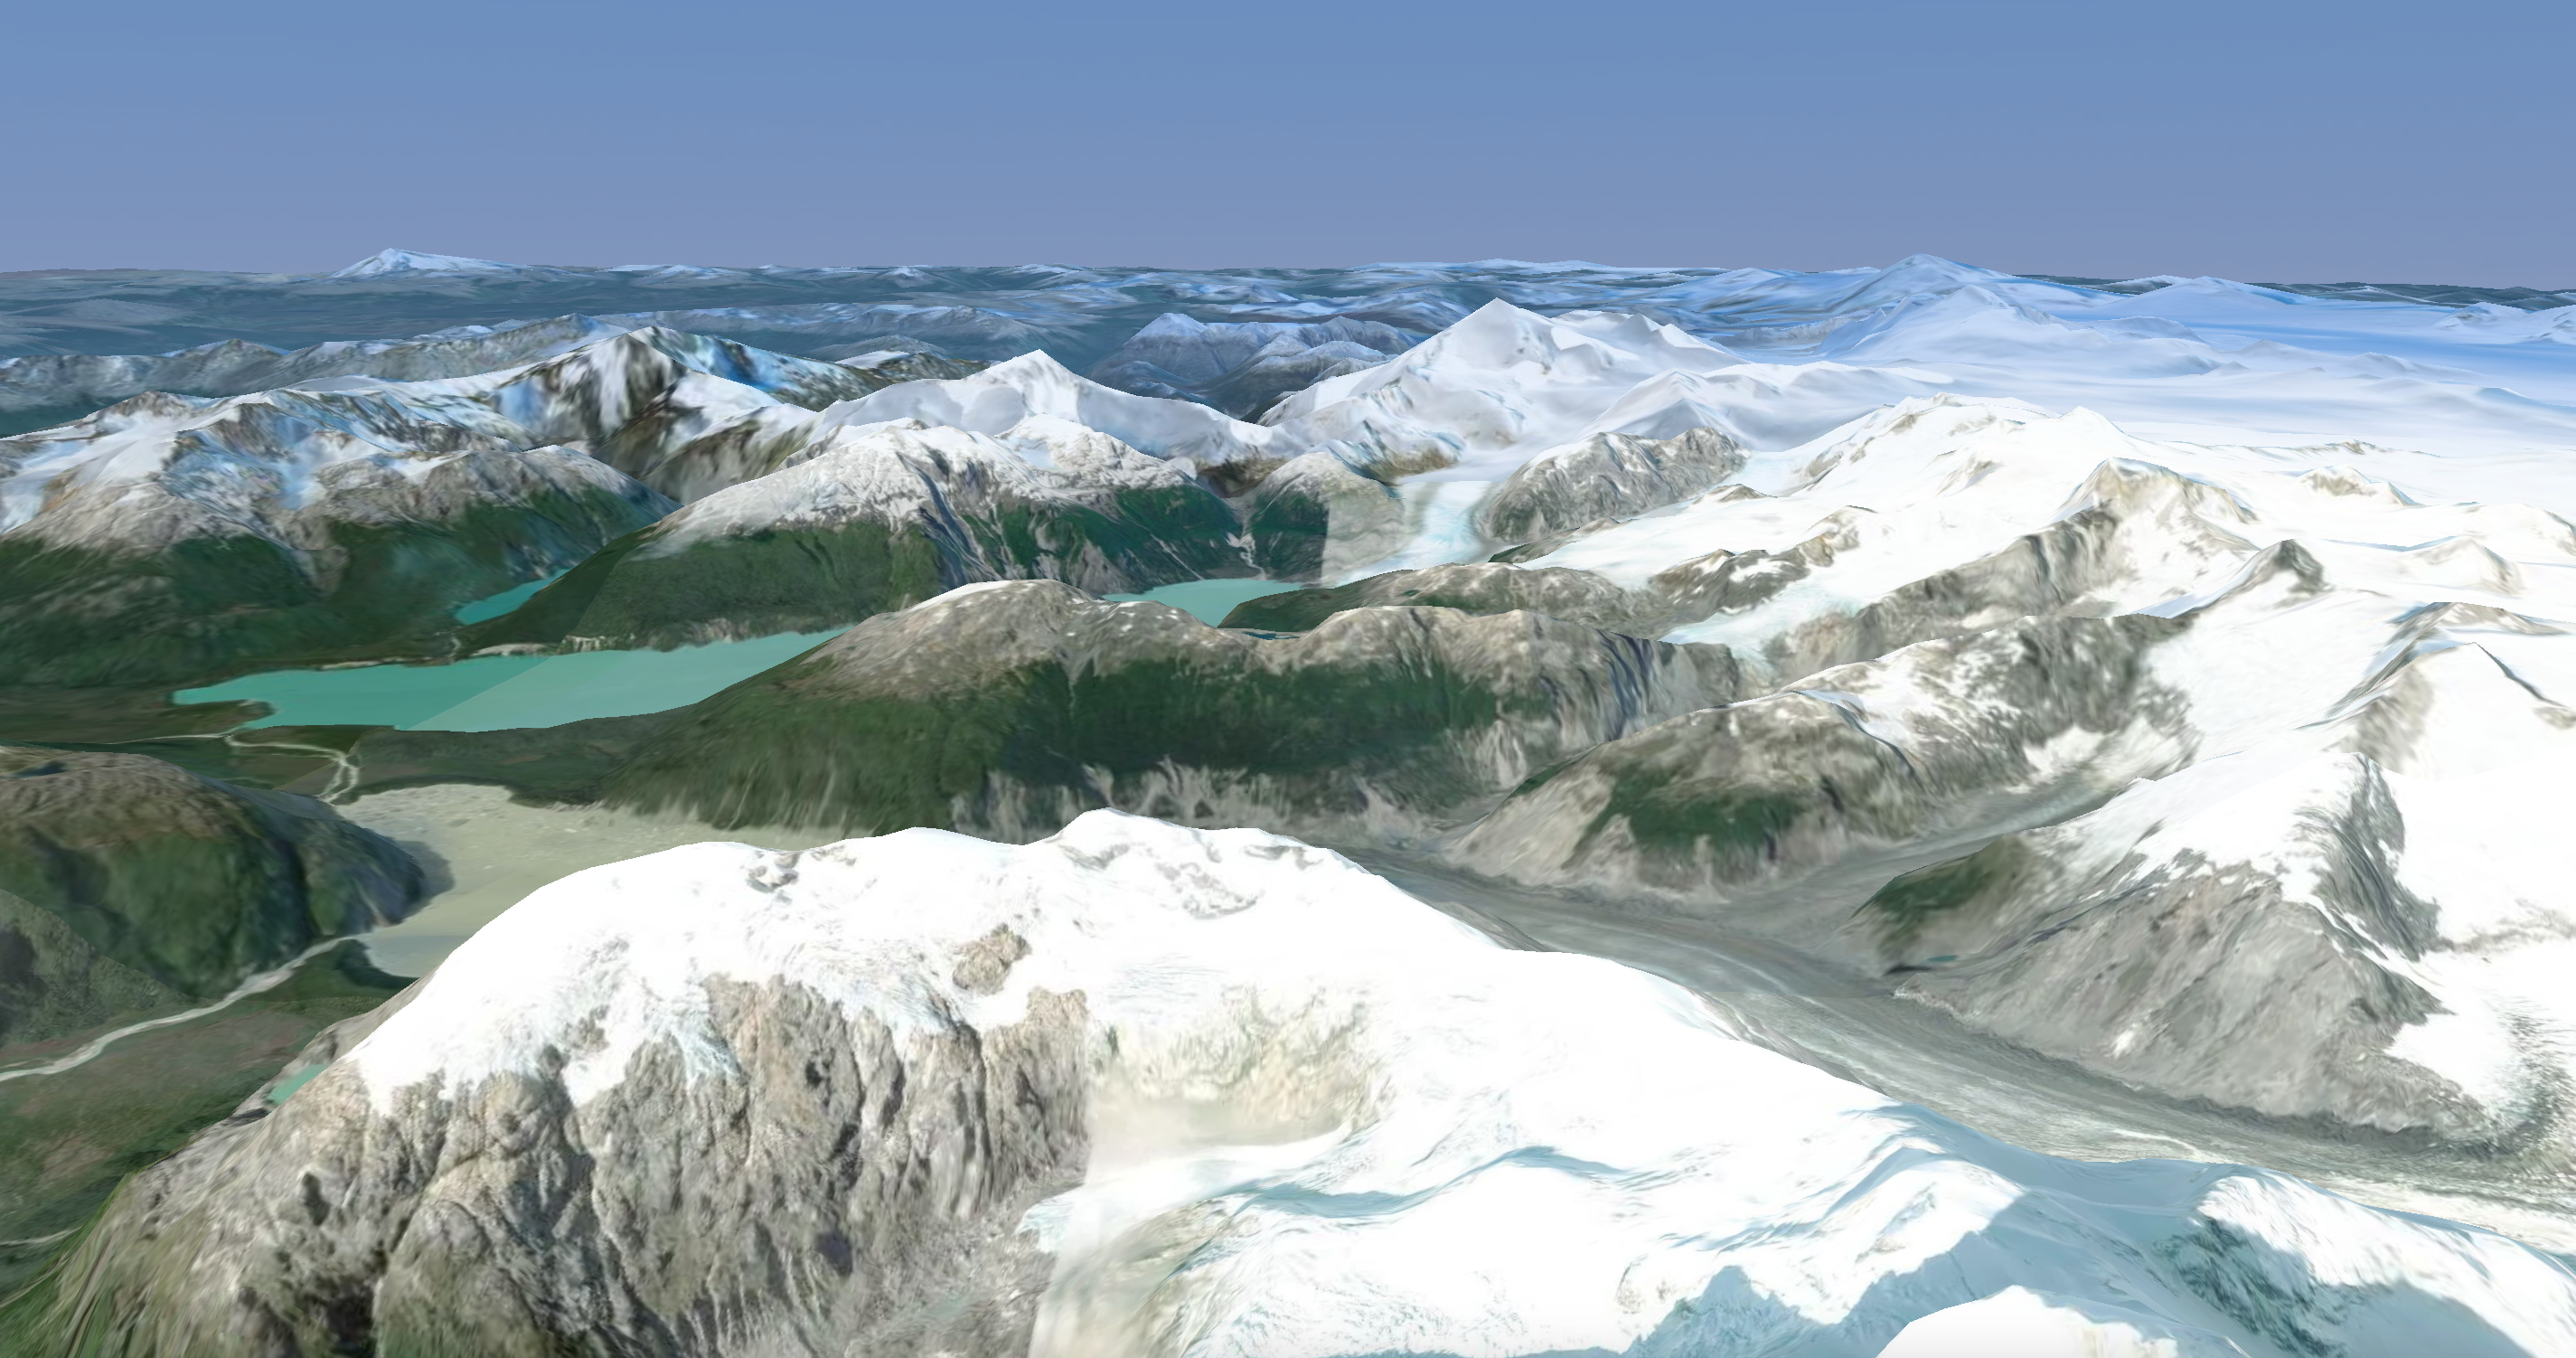
\includegraphics[width=1\textwidth]{results-screenshot-4.png}
  \caption{Screenshot of experiment 4: The Andes mountains.}\label{fig:results-screenshot-4}
\end{figure}

\begin{table}[H]
  \begin{center}
    \begin{tabular}{ c|c }
      Time until destination reached $t_{dest}$ & 30 seconds \\
      \hline
      Time until all tiles loaded $t_{load}$ & 55 seconds \\
      \hline
      $t_{load} - t_{dest}$ & 25 seconds \\
      \hline
      Draw calls & 138 \\
      \hline
      Rendered triangles & 85150 \\
      \hline
      Visible nodes & 68 \\
      \hline
      Traversed nodes & 119 \\
      \hline
      Highest zoom level & 14 \\
      \hline
      Nodes in memory cache & 278 \\
      \hline
      Average FPS & 66.9 \\
      \hline 
      API requests & 626 \\
      \hline
      GPU memory for textures & 509.4 MB \\
      \hline
      Total memory (CPU + GPU) consumption & 1.04 GB \\
    \end{tabular}
  \end{center}
  \caption{Benchmarks for experiment 4.}\label{tbl:results-4}
  \end{table}

\subsection{Experiment 5: The Himalayas}
\begin{figure}[H]
  \centering
  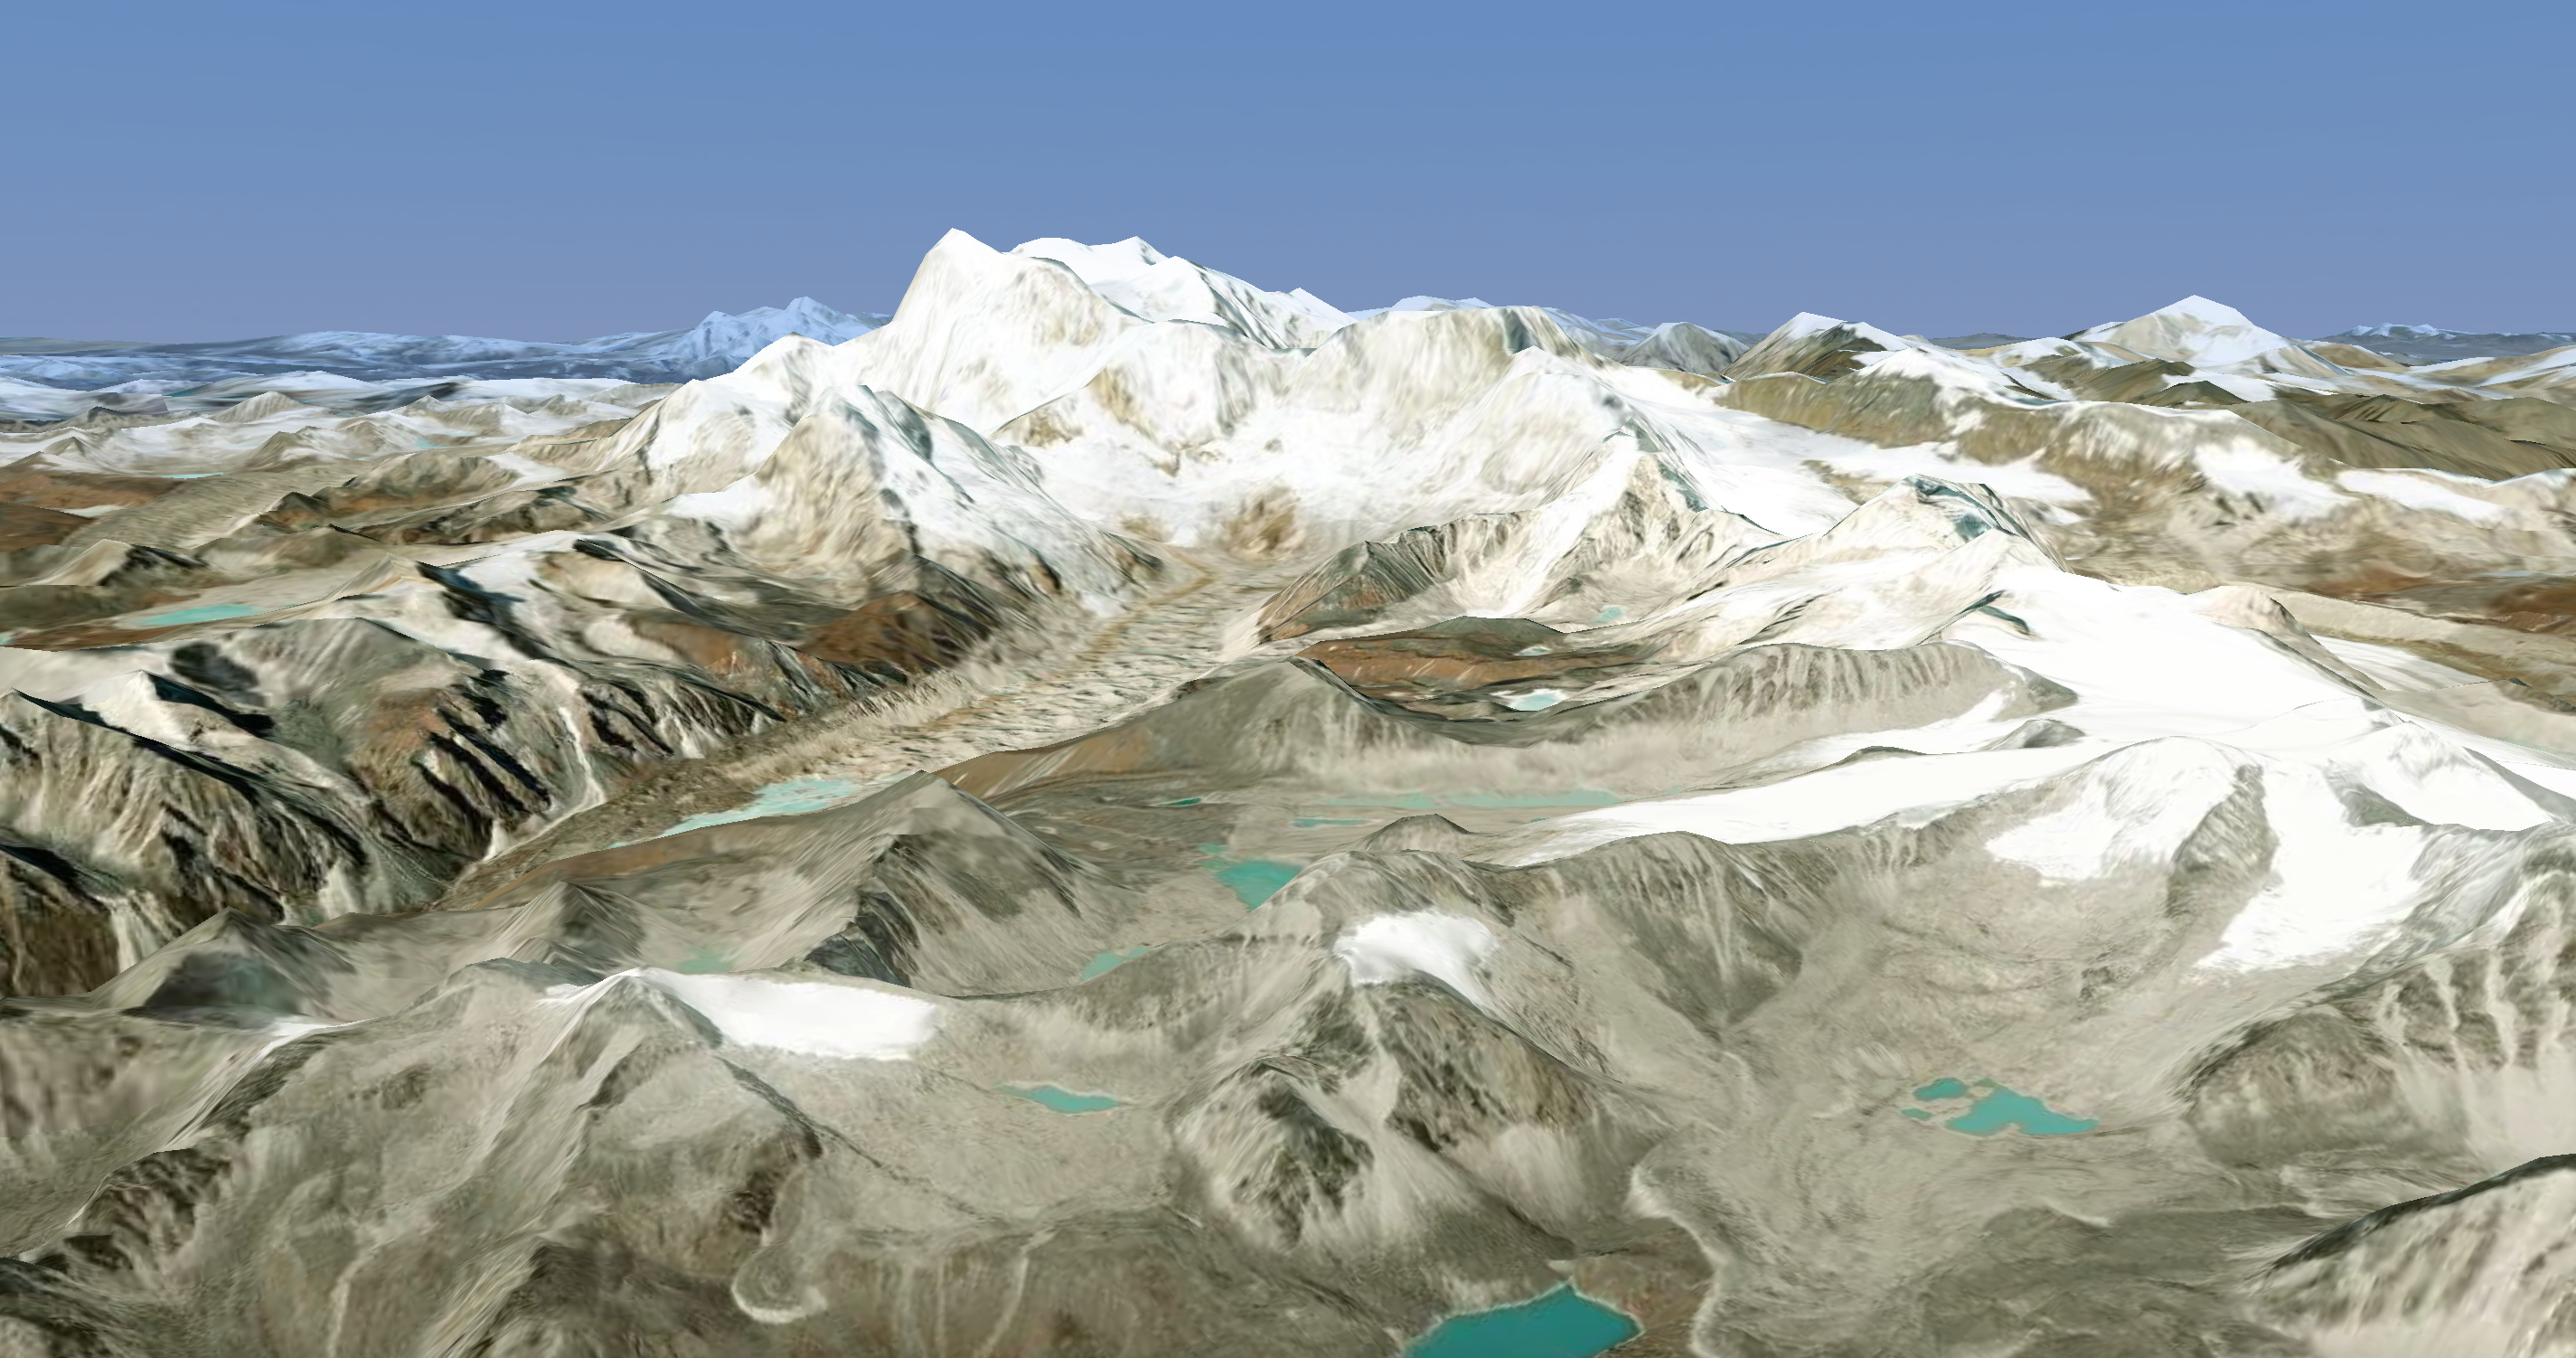
\includegraphics[width=1\textwidth]{results-screenshot-5.png}
  \caption{Screenshot of experiment 5: The Himalayas.}\label{fig:results-screenshot-5}
\end{figure}

\begin{table}[H]
  \begin{center}
    \begin{tabular}{ c|c }
      Time until destination reached $t_{dest}$ & 30 seconds \\
      \hline
      Time until all tiles loaded $t_{load}$ & 46 seconds \\
      \hline
      $t_{load} - t_{dest}$ & 16 seconds \\
      \hline
      Draw calls & 116 \\
      \hline
      Rendered triangles & 78110 \\
      \hline
      Visible nodes & 57 \\
      \hline
      Traversed nodes & 99 \\
      \hline
      Highest zoom level & 14 \\
      \hline
      Nodes in memory cache & 217 \\
      \hline
      Average FPS & 64.5 \\
      \hline 
      API requests & 434 \\
      \hline
      GPU memory for textures & 397.6 MB \\
      \hline
      Total memory (CPU + GPU) consumption & 821.4 MB \\
    \end{tabular}
  \end{center}
  \caption{Benchmarks for experiment 5.}\label{tbl:results-5}
  \end{table}

\subsection{Disk Cache Size Measurements}
\begin{table}[H]
  \begin{center}
    \begin{tabular}{ c|c|c|c }
      Disk cache capacity &  Heightmap subfolder & Overlay subfolder & total \\ 
      \hline
      400 & 74 MB & 18 MB & 92 MB\\
      \hline
      2000 & 311 MB & 93 MB & 404 MB\\
      \hline
      8000 & 1117 MB & 349 MB & 1466 MB = 1.4 GB
    \end{tabular}
  \end{center}
  \caption{Disk cache size measurements for the capacities 400, 2000 and 8000.}\label{tbl:results-disk}
  \end{table}